\documentclass[aspectratio=169,10pt]{beamer}

\usetheme{default}
\usefonttheme{professionalfonts}
\setbeamertemplate{navigation symbols}{}
\setbeamertemplate{footline}{%
  \hfill\scriptsize\insertframenumber/\inserttotalframenumber\hspace{1.2em}\vspace{0.8em}
}
\setbeamertemplate{itemize item}{\raise0.15ex\hbox{\scriptsize$\blacktriangleright$}}
\setbeamertemplate{itemize subitem}{\raise0.15ex\hbox{\scriptsize$\circ$}}

\usepackage[T1]{fontenc}
\usepackage[utf8]{inputenc}
\usepackage{graphicx}
\usepackage{booktabs}
\usepackage{array}
\usepackage{xcolor}
\usepackage{hyperref}

\graphicspath{{figures/}}

\definecolor{Ink}{HTML}{1F2937}
\definecolor{Muted}{HTML}{64748B}
\definecolor{Accent}{HTML}{0F766E}
\definecolor{AccentDark}{HTML}{115E59}
\definecolor{Warm}{HTML}{B45309}
\definecolor{Paper}{HTML}{FBFAF7}
\definecolor{Soft}{HTML}{F3F4F6}

\setbeamercolor{background canvas}{bg=Paper}
\setbeamercolor{normal text}{fg=Ink}
\setbeamercolor{frametitle}{fg=Ink}
\setbeamercolor{title}{fg=Ink}
\setbeamercolor{subtitle}{fg=AccentDark}
\setbeamercolor{structure}{fg=Accent}
\setbeamercolor{alerted text}{fg=Warm}
\setbeamerfont{title}{size=\Large,series=\bfseries}
\setbeamerfont{subtitle}{size=\normalsize}
\setbeamerfont{frametitle}{size=\large,series=\bfseries}
\setbeamerfont{normal text}{size=\normalsize}
\setbeamersize{text margin left=1.1cm,text margin right=1.1cm}

\hypersetup{colorlinks=true,linkcolor=Accent,urlcolor=Accent}

\newcommand{\img}[2][0.88\linewidth]{\includegraphics[width=#1]{#2}}
\newcommand{\code}[1]{\texttt{\small\detokenize{#1}}}

\title{Knowledge-Gap Action Decisions for LLM QA}
\subtitle{An experiment on answer / ask / retrieve / abstain / challenge decisions}
\author{Dayi Yao 2022011550}
\institute{Tsinghua University}
\date{\today}

\begin{document}

\begin{frame}
  \titlepage
\end{frame}

\begin{frame}{Talk Plan}
  \begin{itemize}
    \item Problem: why action selection matters before generation
    \item Project design: data schema, labels, and evaluation targets
    \item Engineering implementation: code structure and main functions
    \item Results: method comparison, ablations, stability, and errors
    \item Limitations: what the current experiment proves and what it does not
  \end{itemize}
\end{frame}

\section{Problem}

\begin{frame}{Problem: Answering Is Only One Possible Action}
  \begin{itemize}
    \item Many user questions are not ready for a final answer.
    \item Missing user constraints call for \alert{asking a question}.
    \item Missing or fresh facts call for \alert{retrieval}.
    \item Unsupported high-stakes claims call for \alert{abstention}.
    \item Contradicted assumptions call for \alert{challenging the premise}.
  \end{itemize}
  \vspace{4mm}
  \Large The project treats this as a supervised action-decision task.
\end{frame}

\begin{frame}{Task Definition}
  \begin{columns}[T,onlytextwidth]
    \column{0.49\textwidth}
    \textbf{Inputs}
    \begin{itemize}
      \item user query
      \item dialogue context
      \item retrieved evidence
      \item candidate answer
    \end{itemize}
    \column{0.49\textwidth}
    \textbf{Outputs}
    \begin{itemize}
      \item \code{gap_type}: explanation label
      \item \code{gold_action}: operational label
      \item action set: answer, ask, retrieve, abstain, challenge
    \end{itemize}
  \end{columns}
\end{frame}

\begin{frame}{Evaluation Target}
  \begin{itemize}
    \item Primary classification metric: action macro-F1.
    \item Safety-sensitive metric: wrong-answer rate.
    \item Utility combines correctness, wrong-answer penalty, over-refusal, over-asking, and turn cost.
    \item The experiment evaluates the next action, not the surface quality of the final long answer.
  \end{itemize}
\end{frame}

\begin{frame}{Related Work Used as Background}
  \begin{itemize}
    \item AmbigQA and ASQA motivate ambiguous-question and clarification cases.
    \item FreshLLMs motivates time-sensitive retrieval decisions.
    \item SelfCheckGPT motivates consistency-style uncertainty features.
    \item Self-RAG motivates retrieval as a controllable action.
    \item Sufficient Context and abstention benchmarks motivate evidence-sufficiency and refusal boundaries.
  \end{itemize}
\end{frame}

\section{Data}

\begin{frame}{Dataset Overview}
  \begin{itemize}
    \item Full run: 800 records generated under controlled knowledge-gap scenarios.
    \item Split: train 483, validation 156, test 161.
    \item Split is by \code{group_id}, so paired variants do not leak across splits.
    \item DeepSeek generation is cached; fallback templates keep the pipeline runnable offline.
  \end{itemize}
\end{frame}

\begin{frame}{Label Distribution}
  \centering
  \img[0.95\linewidth]{label_distribution.png}
\end{frame}

\begin{frame}{Record Schema}
  \begin{itemize}
    \item \code{schema.py} defines \code{GapType}, \code{Action}, required fields, and validation.
    \item Key text fields: \code{user_initial_query}, \code{dialogue_context}, \code{retrieved_evidence}, \code{candidate_answer}.
    \item Key supervision fields: \code{gap_type}, \code{gold_action}, \code{required_slots}.
    \item Annotation fields such as risk and evidence sufficiency are recorded, but not directly used as model features.
  \end{itemize}
\end{frame}

\begin{frame}{Controlled Gap Types}
  \begin{itemize}
    \item \code{sufficient_information}: answer is justified.
    \item \code{ambiguous_question} and \code{user_info_missing}: ask before answering.
    \item \code{evidence_missing} and \code{time_sensitive}: retrieve or abstain depending on the claim.
    \item \code{false_premise}: correct the assumption first.
    \item \code{high_risk_or_expert_needed}: avoid unsupported expert advice.
  \end{itemize}
\end{frame}

\section{Engineering}

\begin{frame}{Repository Structure}
  \begin{itemize}
    \item \code{knowledge_gap_decision/}: core package.
    \item \code{data/processed/}: generated dataset, splits, and feature CSVs.
    \item \code{results/}: metrics, predictions, ablations, significance tests, and figures.
    \item \code{reports/}: generated report and experiment log.
    \item \code{tests/}: schema, leakage, feature, and metric checks.
  \end{itemize}
\end{frame}

\begin{frame}{Data Construction Code}
  \begin{itemize}
    \item \code{build_deepseek_dataset}: calls the JSON-mode DeepSeek client and repairs generated records.
    \item \code{build_dataset}: deterministic fallback dataset generator.
    \item \code{validate_dataset}: catches missing fields, invalid labels, and malformed lists.
    \item \code{split_by_group}: performs leakage-resistant train / val / test split.
    \item \code{write_dataset}: writes JSONL splits and label distribution artifacts.
  \end{itemize}
\end{frame}

\begin{frame}{Feature Extraction Code}
  \begin{itemize}
    \item \code{compute_features}: central feature table builder.
    \item Question-side features: length, time words, condition words, subjective words, entity count, risk keywords.
    \item Evidence-side features: TF-IDF top similarity, token overlap, coverage ratio, contradiction proxy.
    \item Model-side features: offline pseudo-sample agreement, answer variance, majority ratio.
    \item \code{feature_columns}: toggles evidence and uncertainty features for ablations.
  \end{itemize}
\end{frame}

\begin{frame}{Model Code}
  \begin{itemize}
    \item \code{DualClassifier}: trains separate classifiers for \code{gap_type} and \code{gold_action}.
    \item Implemented model kinds: logistic regression, random forest, and GBDT.
    \item \code{TextClassifier}: TF-IDF text-only baseline over query, context, evidence, and candidate answer.
    \item \code{prompted_llm_baseline}: asks DeepSeek for strict JSON action predictions.
    \item \code{full_method_predict}: random-forest prediction plus conservative safety overrides.
  \end{itemize}
\end{frame}

\begin{frame}{Experiment Orchestration}
  \begin{itemize}
    \item \code{run_experiment.run}: one entry point for dataset creation, features, models, metrics, and plots.
    \item \code{_select_full_config}: picks a Full Method variant on validation data.
    \item \code{_write_error_analysis}: writes sampled real mistakes with key feature values.
    \item \code{_write_seed_stability}: reruns the Full Method on three split seeds.
    \item \code{scripts/run_full_experiment.py} and \code{Makefile} provide command-line wrappers.
  \end{itemize}
\end{frame}

\begin{frame}{Evaluation Code}
  \begin{itemize}
    \item \code{evaluate_prediction}: macro-F1, accuracy, retrieval F1, contradiction accuracy, and utility.
    \item \code{utility_components}: wrong-answer rate, over-refusal, over-asking, turn cost.
    \item \code{per_class_rows}: class-level precision / recall / F1 table.
    \item \code{significance_rows}: paired bootstrap and McNemar tests against Full Method.
    \item \code{report.py}: assembles markdown and Word reports from result files.
  \end{itemize}
\end{frame}

\begin{frame}{Question Ranker}
  \begin{itemize}
    \item \code{generate_candidates}: creates clarifying questions from missing slots.
    \item \code{score_question}: combines slot coverage, uncertainty reduction, specificity, answerability, politeness, and leading-question penalty.
    \item \code{rank_questions}: writes \code{results/question_ranker_eval.csv}.
    \item The ranker affects the quality of \code{ask}; it is not the main source of action-F1 gains.
  \end{itemize}
\end{frame}

\begin{frame}{Implementation Caveat}
  \begin{itemize}
    \item Current self-consistency features are generated from offline pseudo samples.
    \item The pseudo-sample generator branches on \code{gap_type}; this makes it a controlled proxy, not a deployable uncertainty estimator.
    \item The ablation is still useful for showing that uncertainty-style signals can separate this dataset.
    \item It should not be described as real black-box LLM self-consistency.
  \end{itemize}
\end{frame}

\section{Results}

\begin{frame}{Main Result: Action Macro-F1}
  \centering
  \img[0.86\linewidth]{method_action_f1.png}
\end{frame}

\begin{frame}{Utility and Wrong-answer Risk}
  \centering
  \img[0.86\linewidth]{utility_wrong_answer.png}
\end{frame}

\begin{frame}{Headline Numbers}
  \begin{itemize}
    \item Full Method: action macro-F1 0.945, action accuracy 0.938.
    \item Full Method: utility 0.875 and wrong-answer rate 0.000.
    \item Always Answer: action macro-F1 0.052, utility -2.404, wrong-answer rate 0.851.
    \item Prompted LLM Baseline: action macro-F1 0.650, wrong-answer rate 0.118.
  \end{itemize}
\end{frame}

\begin{frame}{Per-action F1}
  \centering
  \img[0.94\linewidth]{per_action_f1.png}
\end{frame}

\begin{frame}{Action Confusion Matrix}
  \centering
  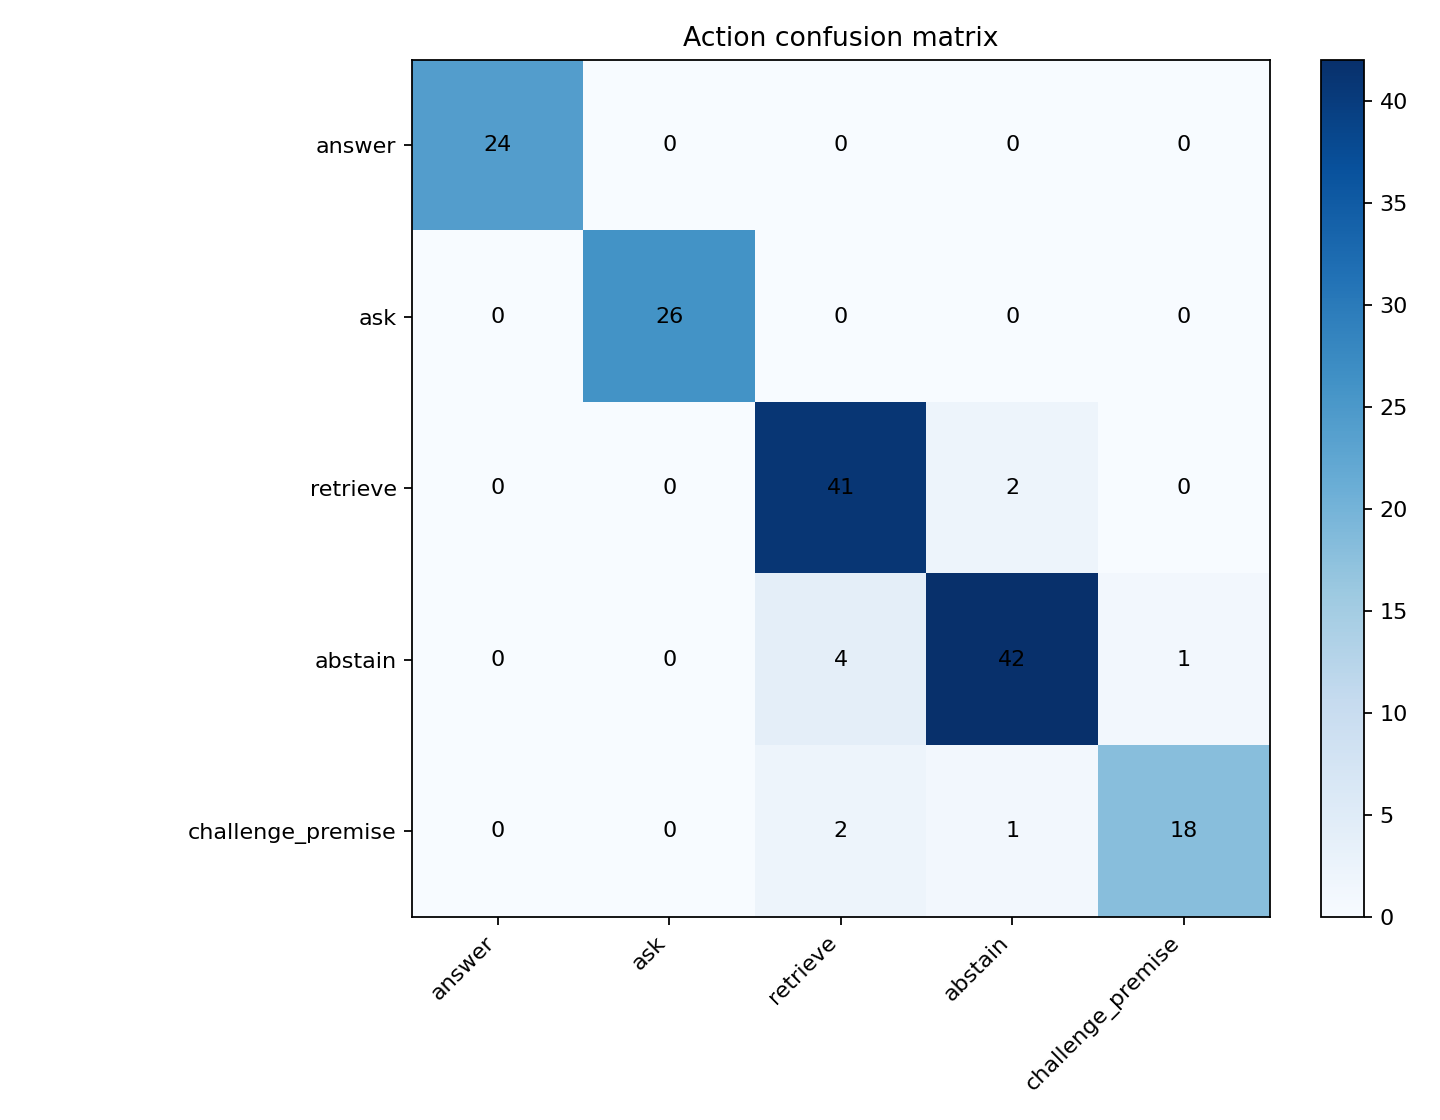
\includegraphics[height=0.72\textheight,keepaspectratio]{confusion_matrix_action.png}
\end{frame}

\begin{frame}{Gap-type Confusion Matrix}
  \centering
  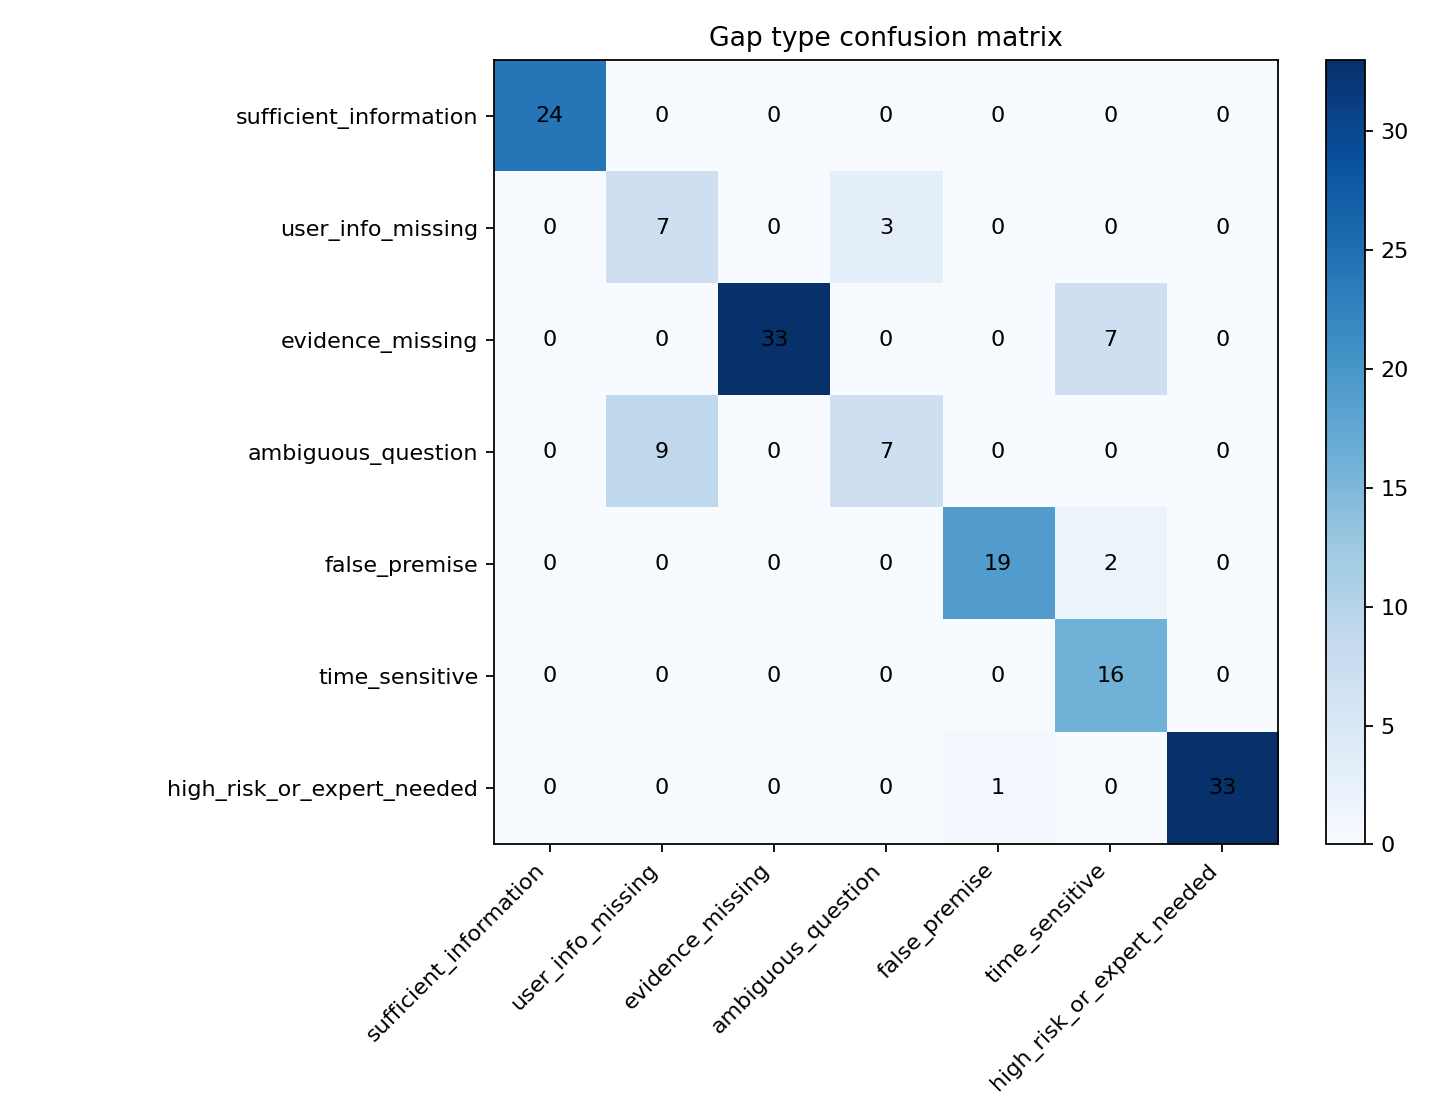
\includegraphics[height=0.72\textheight,keepaspectratio]{confusion_matrix_gap_type.png}
\end{frame}

\begin{frame}{Validation Selection}
  \centering
  \img[0.78\linewidth]{validation_selection.png}
\end{frame}

\begin{frame}{Ablation}
  \centering
  \img[0.88\linewidth]{ablation_delta.png}
\end{frame}

\begin{frame}{Significance Tests}
  \centering
  \img[0.88\linewidth]{significance_forest.png}
\end{frame}

\begin{frame}{Repeated Split Stability}
  \centering
  \img[0.78\linewidth]{stability.png}
\end{frame}

\begin{frame}{Residual Errors}
  \centering
  \img[0.76\linewidth]{error_categories.png}
\end{frame}

\section{Case Discussion}

\begin{frame}{Example Boundaries}
  \begin{itemize}
    \item Ambiguous technical question: ask about environment and target before giving steps.
    \item Current policy or deadline: retrieve fresh evidence before answering.
    \item False premise: state that the assumption is unsupported before continuing.
    \item Evidence-support judgment: abstain if the supplied evidence does not support the claim.
  \end{itemize}
\end{frame}

\begin{frame}{What the Results Say}
  \begin{itemize}
    \item Explicit action labels are much safer than default answering.
    \item Structured features beat direct prompted classification on this controlled dataset.
    \item Full Method is close to Random Forest and GBDT; its advantage over them is not statistically strong.
    \item The largest ablation drop comes from removing uncertainty-style features.
  \end{itemize}
\end{frame}

\begin{frame}{Limitations}
  \begin{itemize}
    \item The dataset is generated under controlled scenarios, not collected from real users.
    \item Some labels may still reflect the generator's style and scenario design.
    \item Evidence contradiction is handled by a heuristic proxy, not a strong NLI verifier.
    \item The current uncertainty feature is not real multi-sample LLM uncertainty.
  \end{itemize}
\end{frame}

\begin{frame}{Next Steps}
  \begin{itemize}
    \item Add real user questions and human label adjudication.
    \item Replace offline pseudo-consistency with real multi-sample uncertainty or calibrated model confidence.
    \item Add harder adjacent-label examples, especially retrieve vs abstain and false premise vs time-sensitive.
    \item Test out-of-distribution domains and generation models.
  \end{itemize}
\end{frame}

\begin{frame}{Takeaway}
  \Large
  A reliable QA system should decide whether answering is justified before it writes the answer.
  \vspace{6mm}

  \normalsize
  This project provides a reproducible prototype for modeling that decision, with clear evidence and clear limits.
\end{frame}

\begin{frame}{References}
  \footnotesize
  \begin{itemize}
    \item Min et al. AmbigQA: Answering Ambiguous Open-domain Questions. EMNLP 2020. \href{https://arxiv.org/abs/2004.10645}{arXiv:2004.10645}
    \item Stelmakh et al. ASQA: Factoid Questions Meet Long-Form Answers. EMNLP 2022. \href{https://arxiv.org/abs/2204.06092}{arXiv:2204.06092}
    \item Vu et al. FreshLLMs: Refreshing Large Language Models with Search Engine Augmentation. 2023. \href{https://arxiv.org/abs/2310.03214}{arXiv:2310.03214}
    \item Manakul et al. SelfCheckGPT: Zero-Resource Black-Box Hallucination Detection. 2023. \href{https://arxiv.org/abs/2303.08896}{arXiv:2303.08896}
    \item Asai et al. Self-RAG: Learning to Retrieve, Generate, and Critique through Self-Reflection. 2023. \href{https://arxiv.org/abs/2310.11511}{arXiv:2310.11511}
    \item Sufficient Context: A New Lens on Retrieval Augmented Generation Systems. 2024. \href{https://arxiv.org/abs/2411.06037}{arXiv:2411.06037}
    \item Kirichenko et al. AbstentionBench: Reasoning LLMs Fail on Unanswerable Questions. 2025. \href{https://arxiv.org/abs/2506.09038}{arXiv:2506.09038}
  \end{itemize}
\end{frame}

\end{document}
